\section{Fault Injection using Software Tools}

Software-Implemented Fault Injection (SWIFI) has become a prominent technique for evaluating system reliability, particularly as hardware complexity increases and physical access to internal components becomes more difficult. Unlike hardware-based methods that require physical probes or radiation sources, SWIFI emulates hardware faults by modifying software states, memory contents, or register values during program execution.

\subsection{Overview of SWIFI Techniques}
SWIFI techniques are generally classified into two main categories: compile-time and runtime injection. Compile-time injection involves modifying the source code or assembly code to insert fault triggers before the program is built. Runtime injection, which is largely more common, uses mechanisms such as interrupts, debuggers, or exception handlers to intercept program execution and alter the state of the processor or memory.

Common targets for SWIFI include:
\begin{itemize}
    \item \textbf{CPU Registers:} Corrupting general-purpose or special-purpose registers to simulate transient CPU faults.
    \item \textbf{Memory:} Flipping bits in  text code, data, heap, or stack segments to emulate Single Event Upsets (SEUs) in RAM.
    \item \textbf{I/O Interfaces:} Intercepting and corrupting data packets to test communication protocols.
\end{itemize}

SWIFI is highly valued for its low cost, flexibility, and ability to target specific software structures. However, it suffers from intrusiveness, as the injection code itself adds overhead, potentially missing real-world timing issues, making it less useful for sensitive real-time systems.

\subsection{Case Study: Failure Assessment of NASA cFS Case-Study Flight Software on RISC-V via Fault Injection}
A recent study by Fran\c{c}a et al. \cite{SoftwareSite} demonstrates the application of SWIFI to assess the reliability of safety-critical flight software. This case study evaluates NASA's Core Flight System (cFS), a reusable software framework used in missions like the Lunar Reconnaissance Orbiter and the James Webb Space Telescope, running on a RISC-V PolarFire System-on-Chip (SoC).

The study utilized a fault injection campaign to simulate radiation-induced faults in Low Earth Orbit (LEO). The experimental setup involved a RISC-V PolarFire SoC running the FreeRTOS operating system with a port of NASA's Operating System Abstraction Layer (OSAL). Faults were injected into the volatile memory (RAM) where application data, stack, and heap were stored. A Python-based host script communicated with the target via a serial port interrupt to trigger bit-flips at random memory addresses and time intervals. As the workload, two benchmark applications were used as probes: Huffman encoding/decoding and Fixed-Point Matrix Multiplication.

\begin{figure}[htbp]
    \centering
    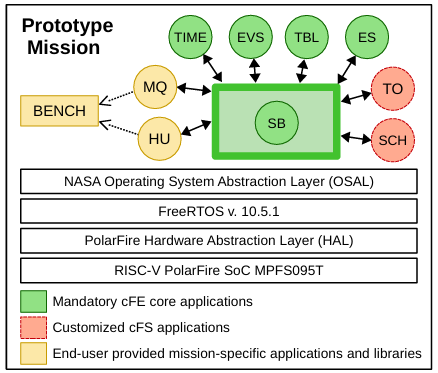
\includegraphics[width=0.75\linewidth]{assets/Mission software stack.png}
    \caption{Mission software stack}
    \label{fig:Mission}
\end{figure}

The campaign observed 2,270 functional failures, classifying them into three categories: I/O Timeouts (system hang), Silent Data Corruption (SDC) and Result Timeouts. Approximately 79\% of the observed failures resulted in the flight software becoming unresponsive (I/O Timeout), requiring a hardware reset. The system remained active but produced incorrect results 12\% of the time (SDC) and it transmitted data that could not be decoded 9\% of the time
(Result Timeout).

By utilizing FreeRTOS trace resources, the study identified that the cFS Scheduler (SCH) task was the most sensitive to faults. Failures during the SCH task execution accounted for over 21\% of the total failures. The study mapped failure rates to specific memory footprints. For instance, the Event Services (EVS) task, despite having a small footprint, showed a disproportionately high number of failures, indicating high architectural vulnerability.

\begin{figure}[htbp]
    \centering
    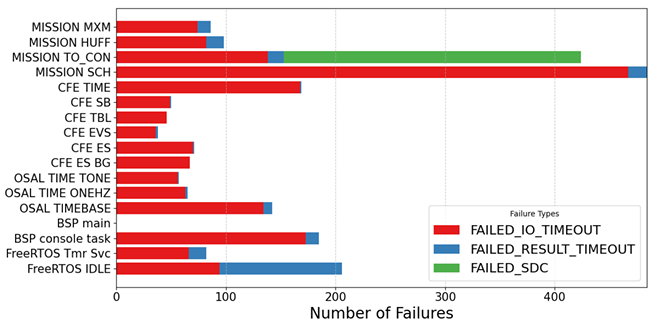
\includegraphics[width=0.9\linewidth]{assets/SWIFI_failures.png}
    \caption{Number of Failures detected while the task was executing.}
    \label{fig:SWIFI_failures}
\end{figure}

This case study illustrates how SWIFI can effectively identify critical software modules (e.g., the Scheduler) that require hardening, enabling targeted fault tolerance improvements without the need for expensive radiation testing facilities. Furthermore, it demonstrated the viability of NASA's cFS framework on open source platforms such as RISC-V and FreeRTOS.